\chapter{Simulate 2D Brownian motion of $\textbf{\textit{E.coli}}$ with constant chemoattractant(A) gradient along x-direction} % Main chapter title

\label{Part1_chapter} % For referencing the chapter elsewhere, use \ref{Chapter1} 

\section{Symbols}

\begin{table}[H]
\caption{The symbols used in the model of simulating simple 2D Brownian motion of $E.coli$ with constant chemoattractant(A) gradient along x-direction }
\label{tab:part2_symbols}
\centering
\begin{tabular}{l l}
\toprule

\tabhead{Symbol} & \tabhead{Definition} \\
\midrule
$N(\mu,\sigma)$ & Normal distribution with mean $\mu$ and standard deviation $\sigma$ \\
% ${\rm R^{2}_{i}}$ 改成正常体
$\Delta x$ & Space interval \\
$\Delta t$ & Time interval \\
$\qquad \sigma  $ & $\qquad \sigma = \Delta x$/$\sqrt{ \Delta t}$ \\
$(x,y)$ & Coordinates of $E.coli$ \\
$\qquad x_t  $ & \qquad Coordinate in x axis at time t \\
$\qquad y_t  $ & \qquad Coordinate in y axis at time t \\
$v$			   & The speed of the movement of $E.coli$ \\
$A$		       & The chemoattractant \\
$A_0$		   & The chemoattractant at $x=0$ \\
$k$			   & Gradient of chemoattractant along x-direction \\ 
\bottomrule\\
\end{tabular}
\end{table}

\newpage
\section{Hypothesize our own chemotaxis actions}
\begin{equation*} 
\begin{aligned} 
\centering
A(x) &= A_0 + kx \\
\end{aligned} 
\end{equation*}

\section{Hypothesis for simulation}

Assuming the $E.coli$ here have no mitosis, so the number of cells maintain constant.
I use $(x,y)$ to define the location of each cell, assume all the cells start from origin$(0,0)$. They have a random judging for each step in both x and y directions. Set the speed as $50 \mu m/s$, so for each step,

\begin{equation*} 
\begin{aligned} 
\centering
\phi_x &\backsim N(0,1) \\
\phi_y &\backsim N(0,1) \\
x_{t+1}  &=  x_{t} + \phi_x v + max[(A_0 + kx_t),0]\\ 
y_{t+1}  &=  y_{t} + \phi_y v \\ 
\end{aligned} 
\end{equation*}

%----------------------------------------------------------------------------------------
%\newpage
\section{Results of simulation}

\begin{figure}[H]
\centering
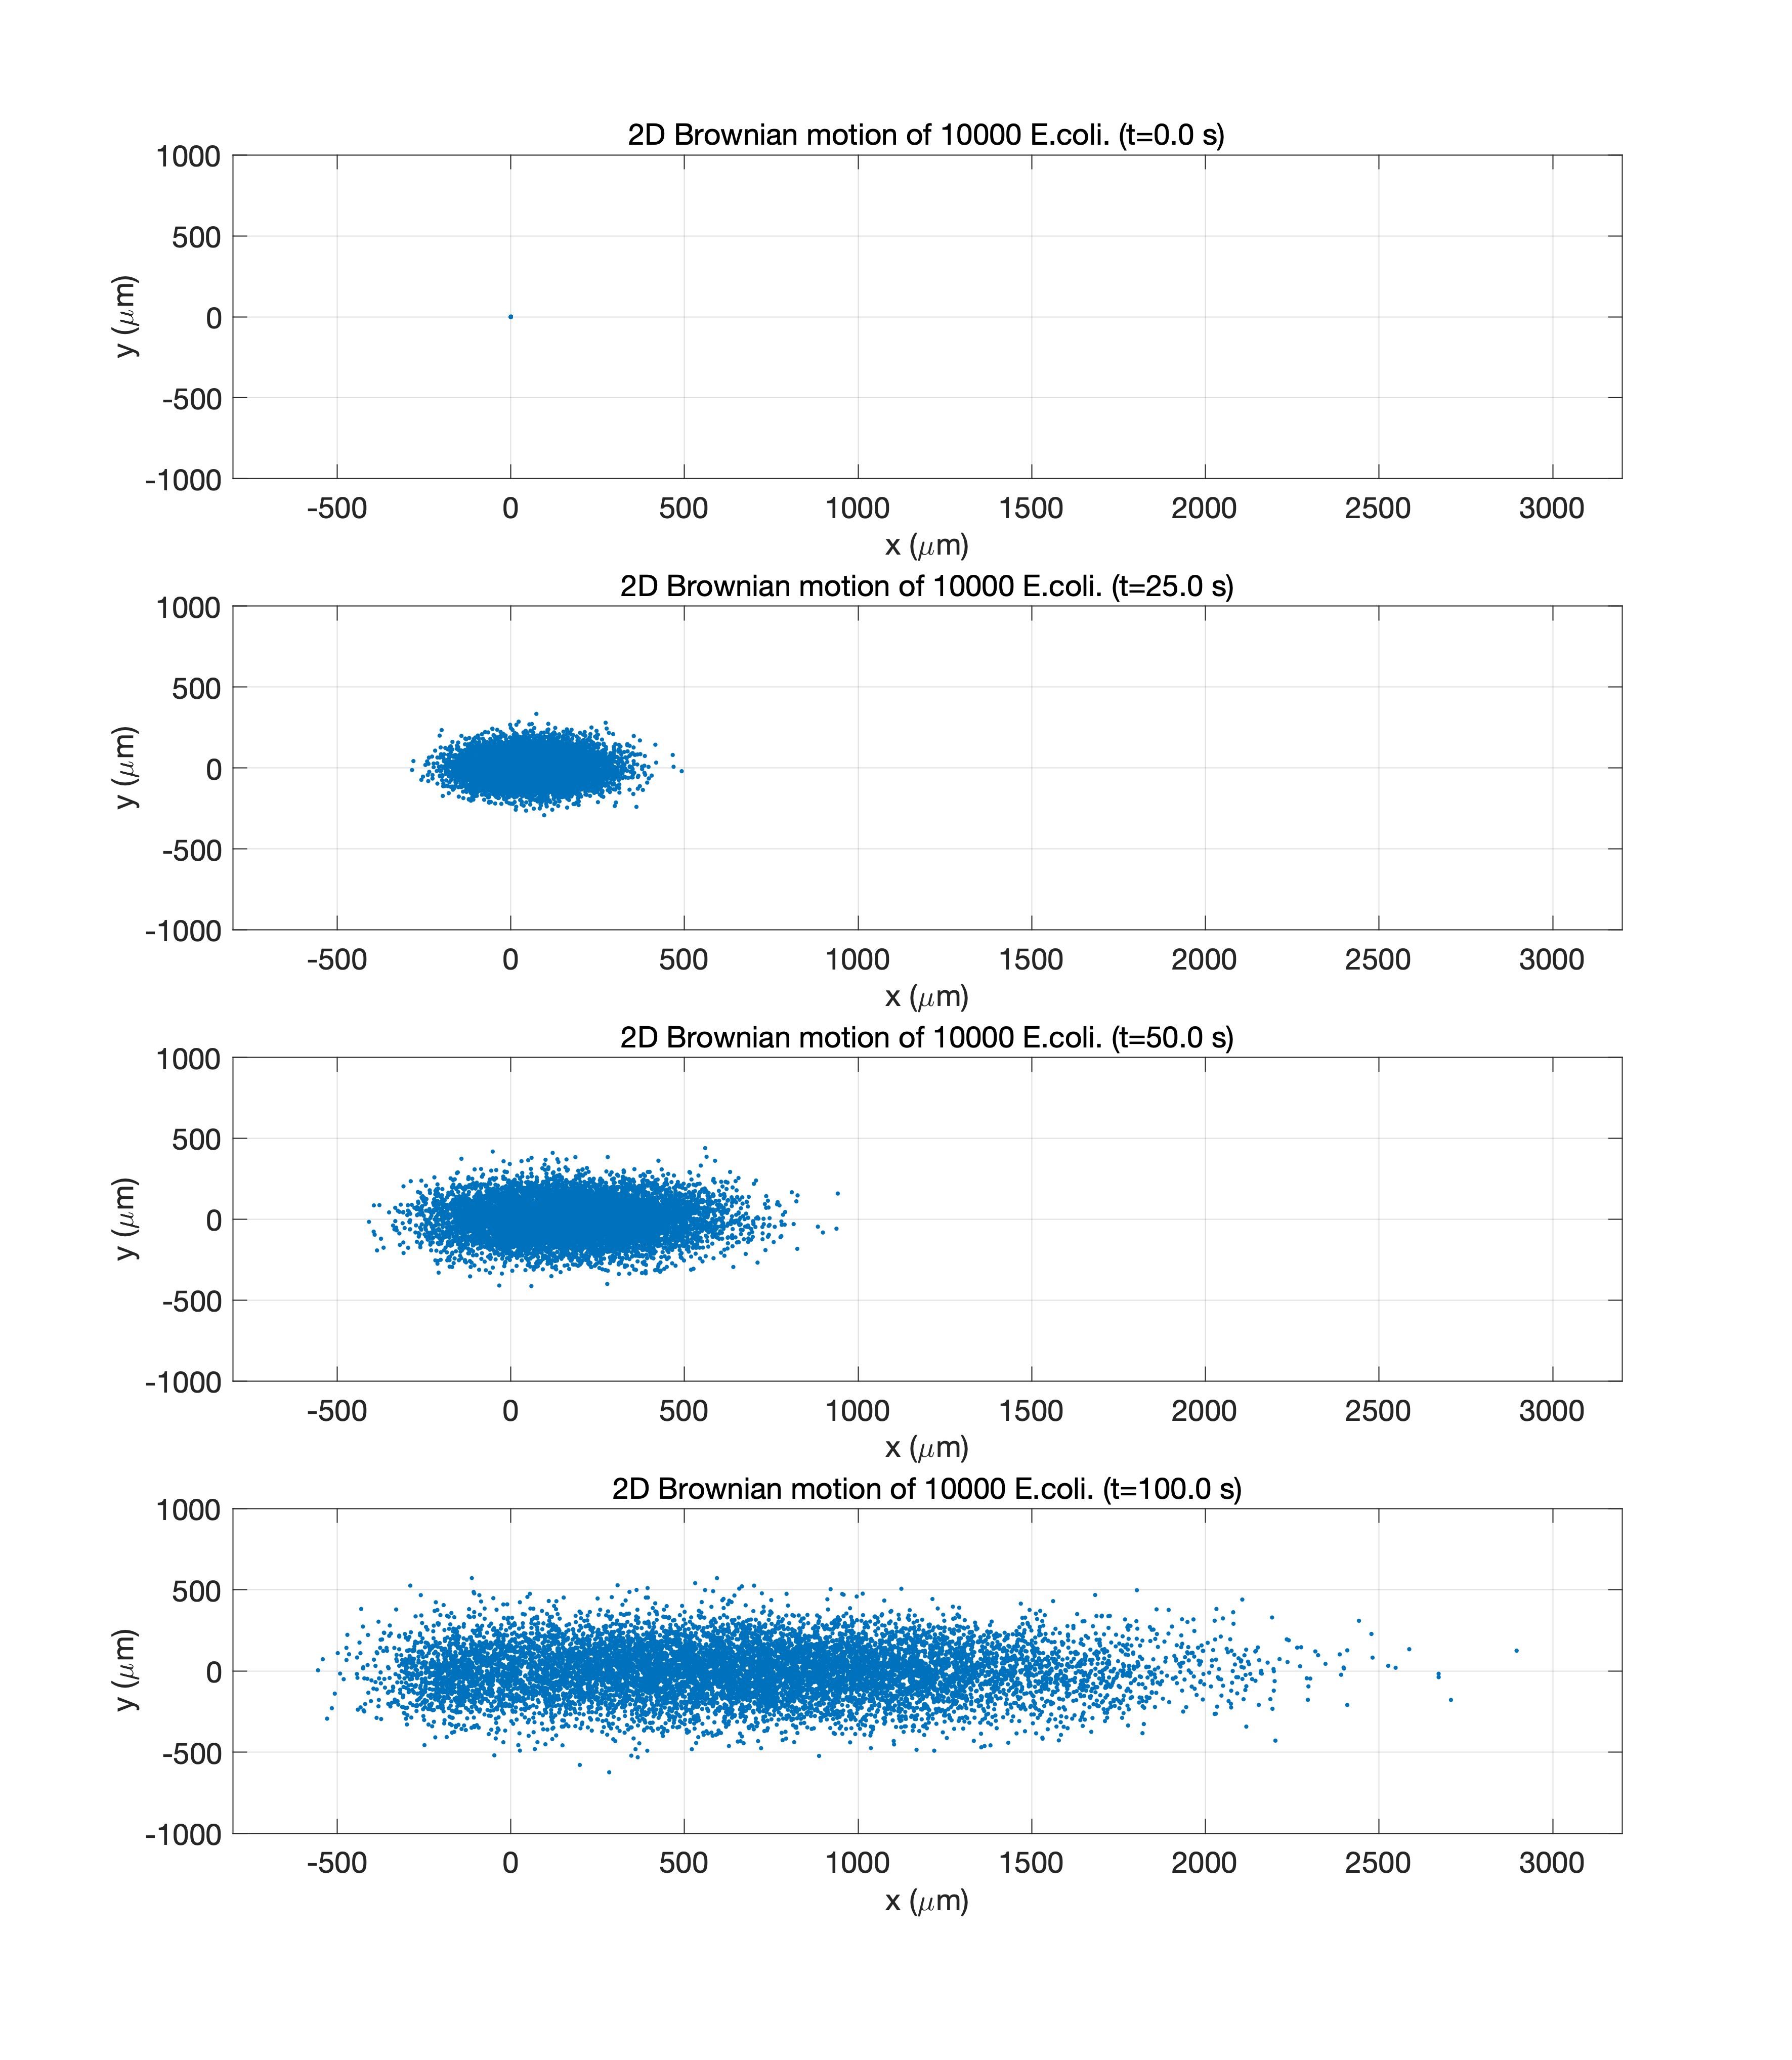
\includegraphics[width=1\linewidth]{Figures/P2_fig1.png}
\caption{The simulation of 10000 $E.coli$ cells for simple 2D Brownian motion with constant chemoattractant gradient along X-direction form $(0,0)$ after 100s \\
** $A_0=2\mu m$ and $k=0.02$}
\label{P2_fig1}
\end{figure}

\begin{figure}[H]
\centering
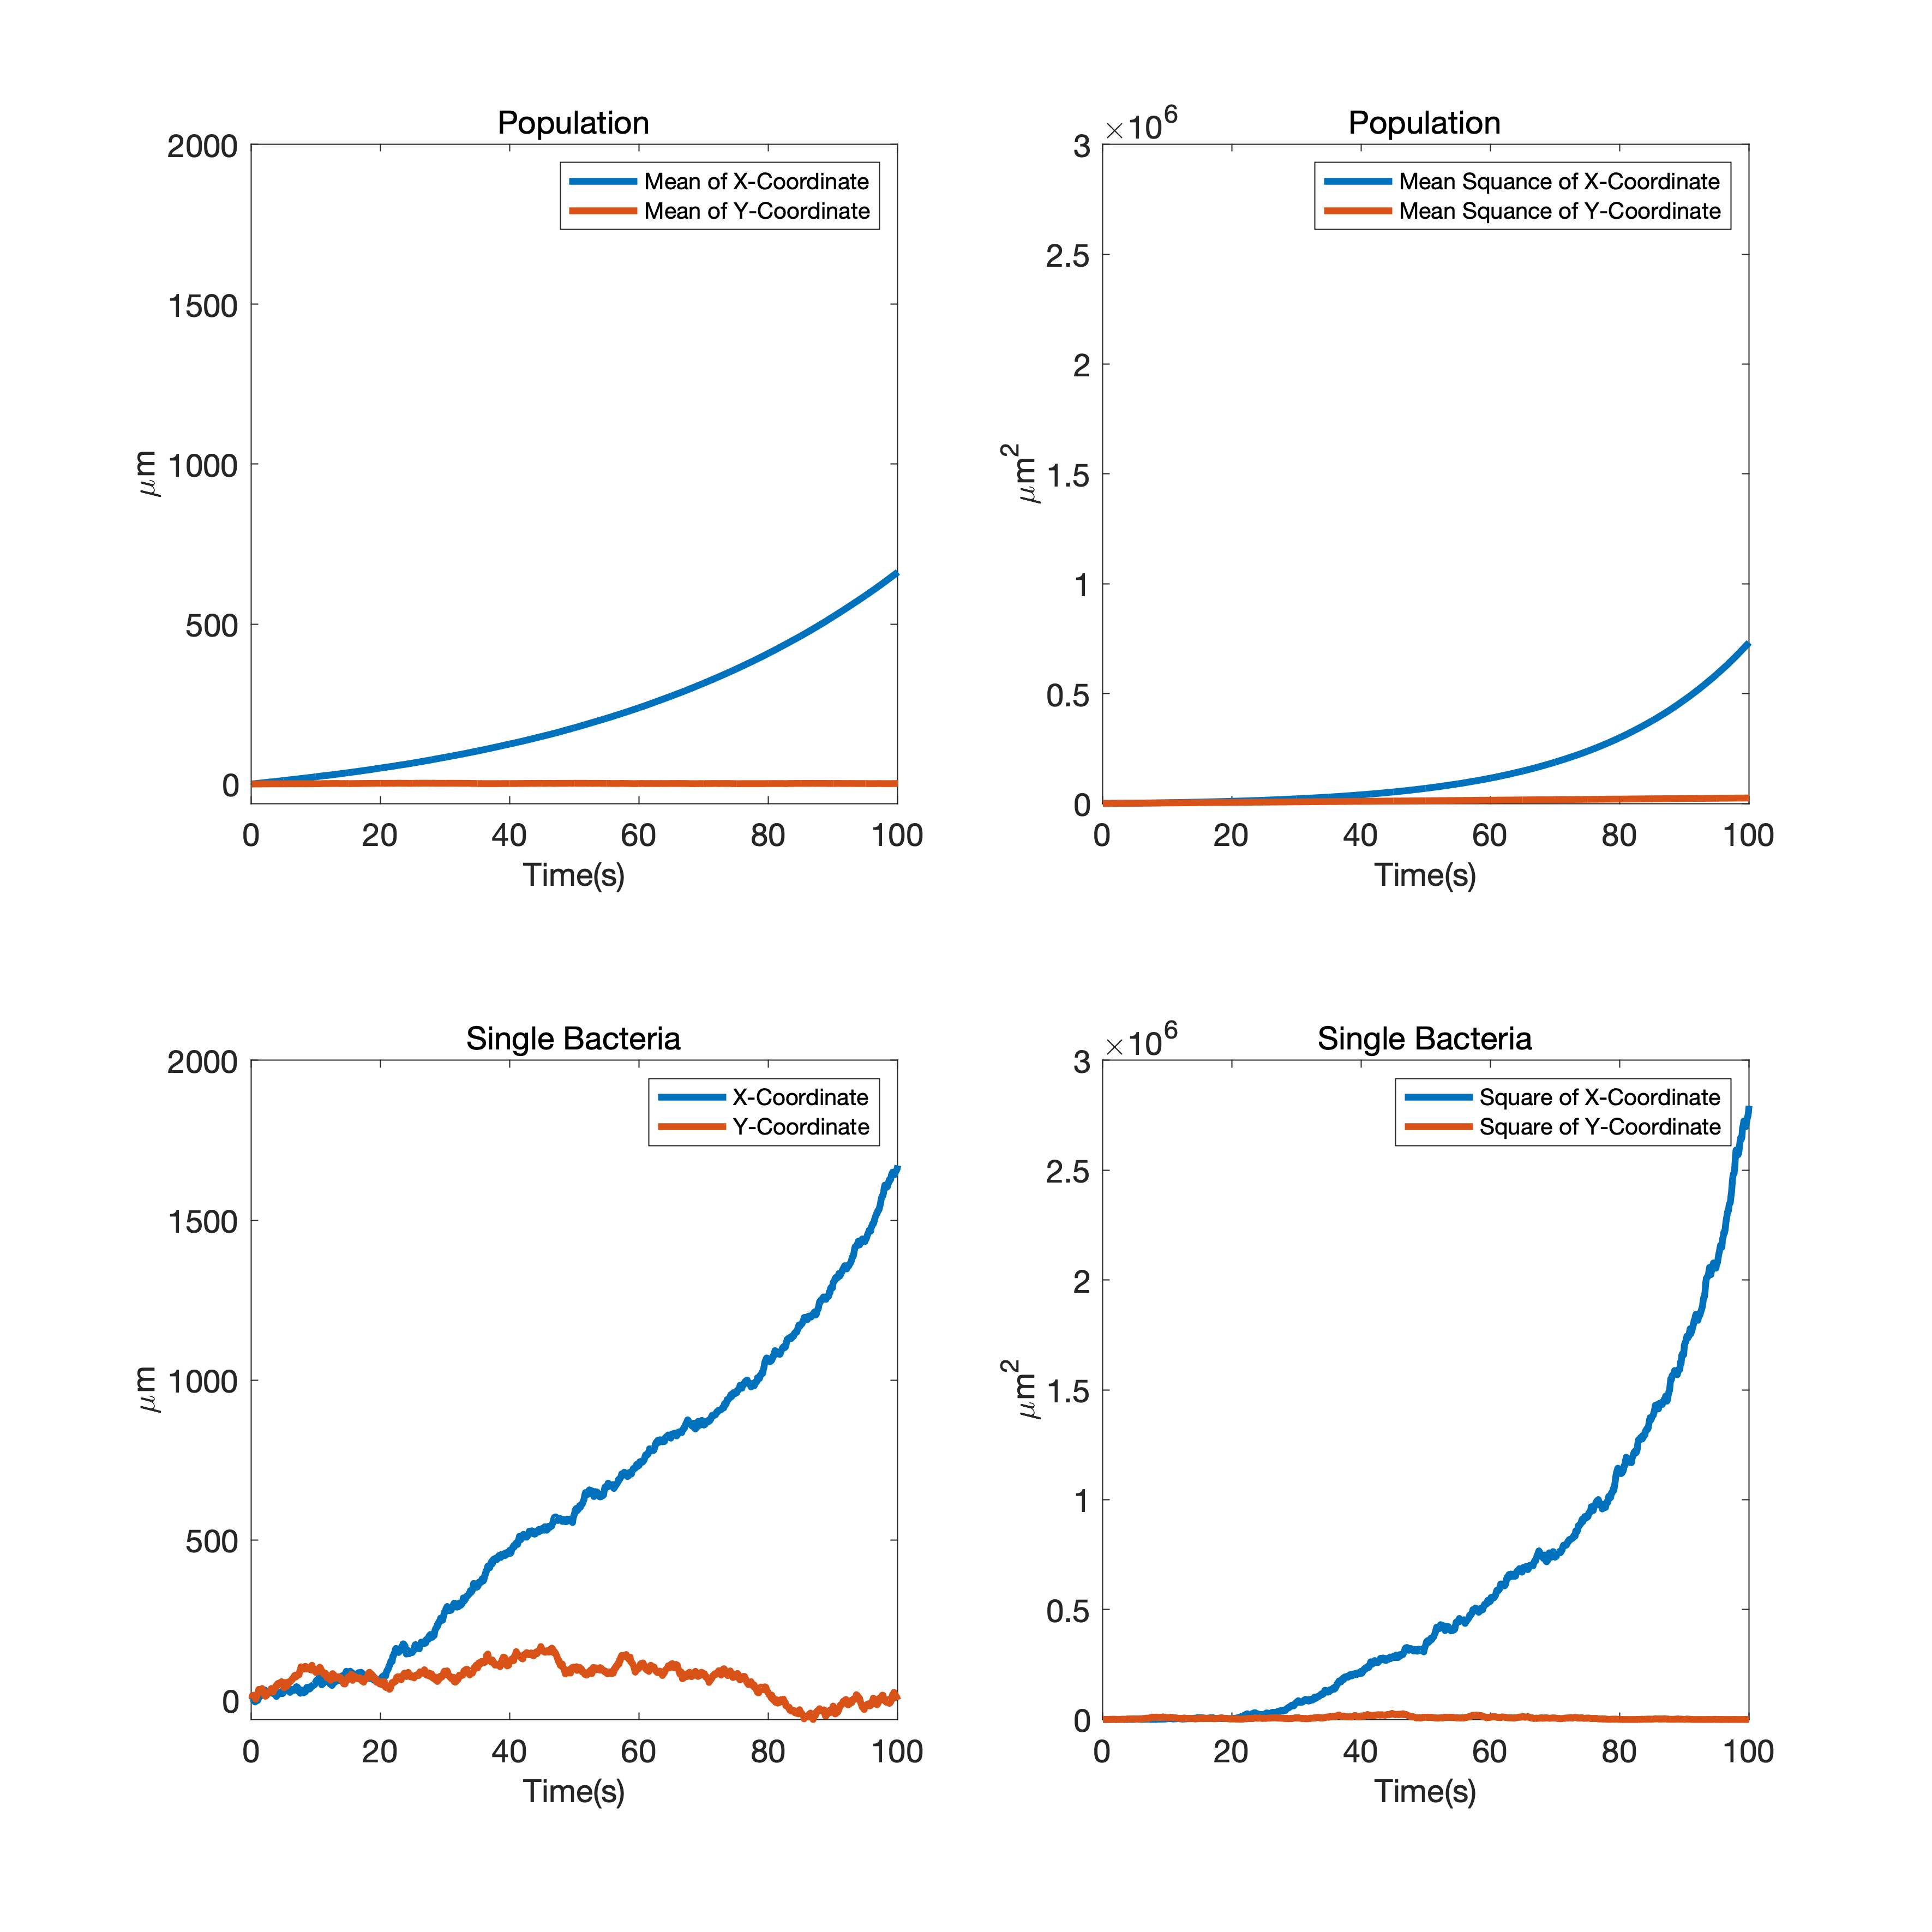
\includegraphics[width=1\linewidth]{Figures/P2_fig2.png}
\caption{The ”mean displacement” and ”mean displacement-square” overtime for simple 2D brownic motion}
\label{P2_fig2}
\end{figure}


\begin{figure}[H]
\centering
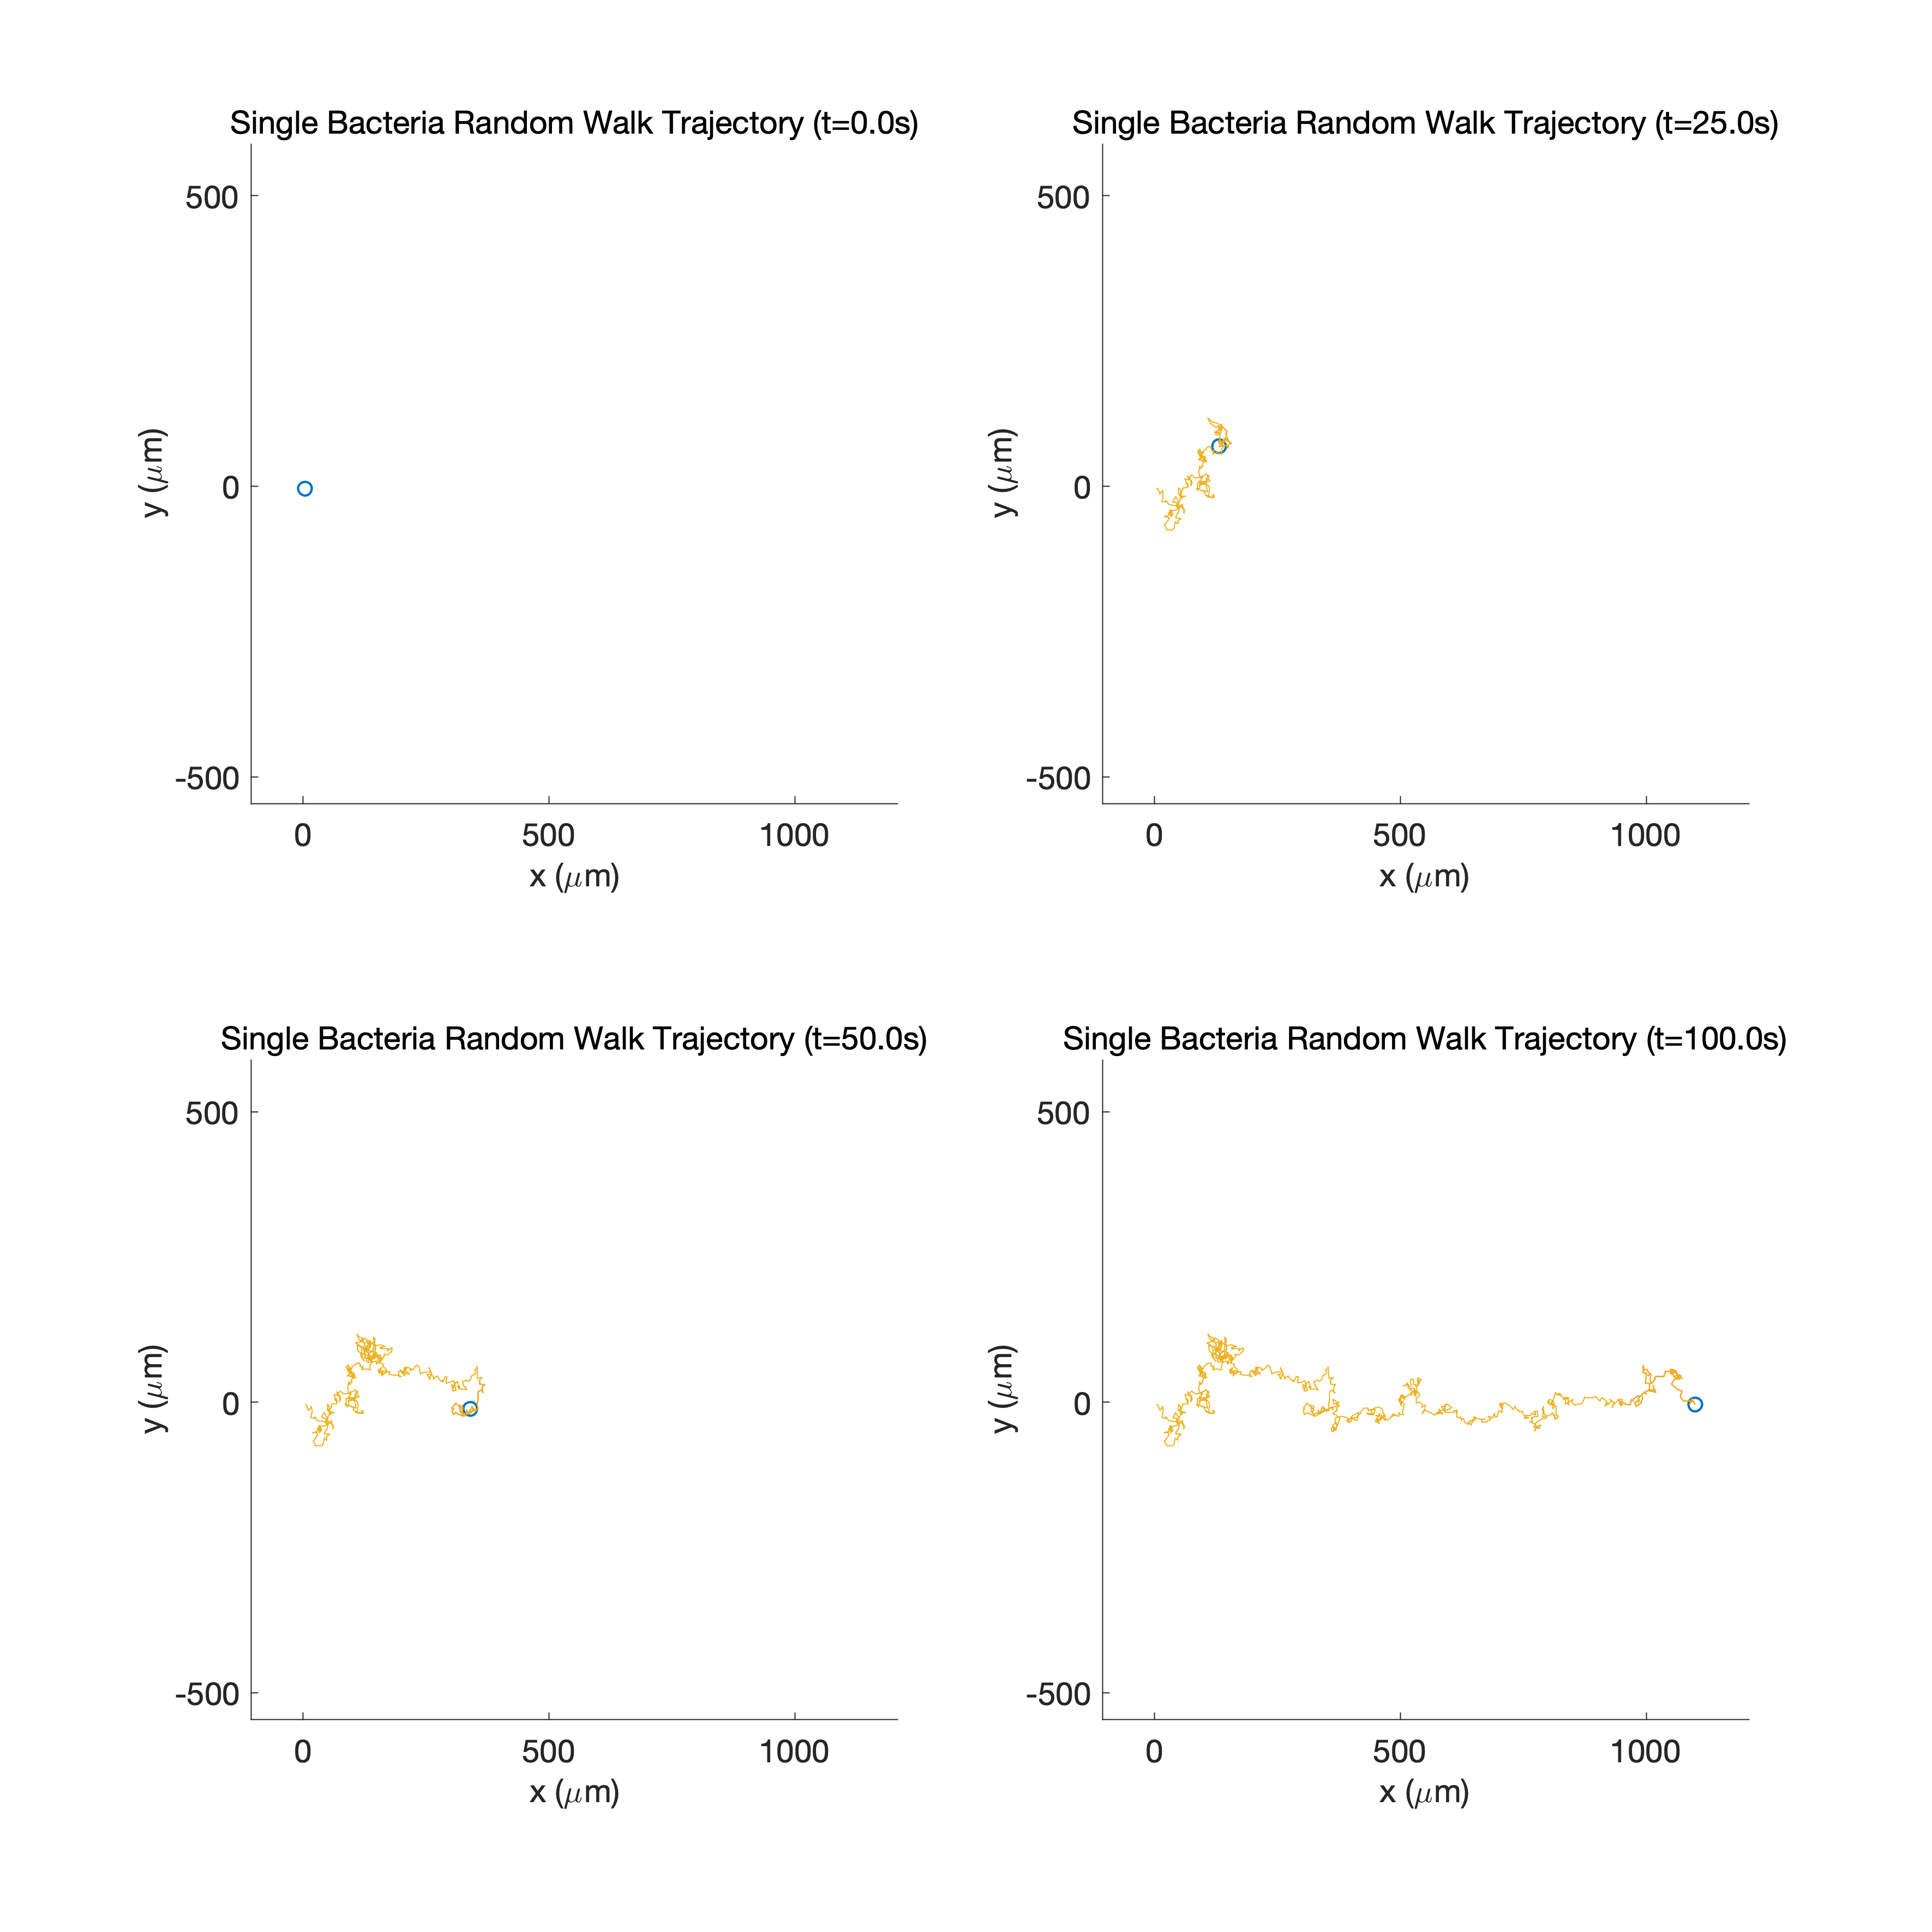
\includegraphics[width=1\linewidth]{Figures/P2_fig3.png}
\caption{Single Bacteria Random Walk Trajectory}
\label{P2_fig3}
\end{figure}


%----------------------------------------------------------------------------------------

\section{Comparing ``simple Brownian motion'' and ``Brownian motion with chemotaxis in x-direction'' for 10000 cells.}

\begin{figure}[H]
\centering
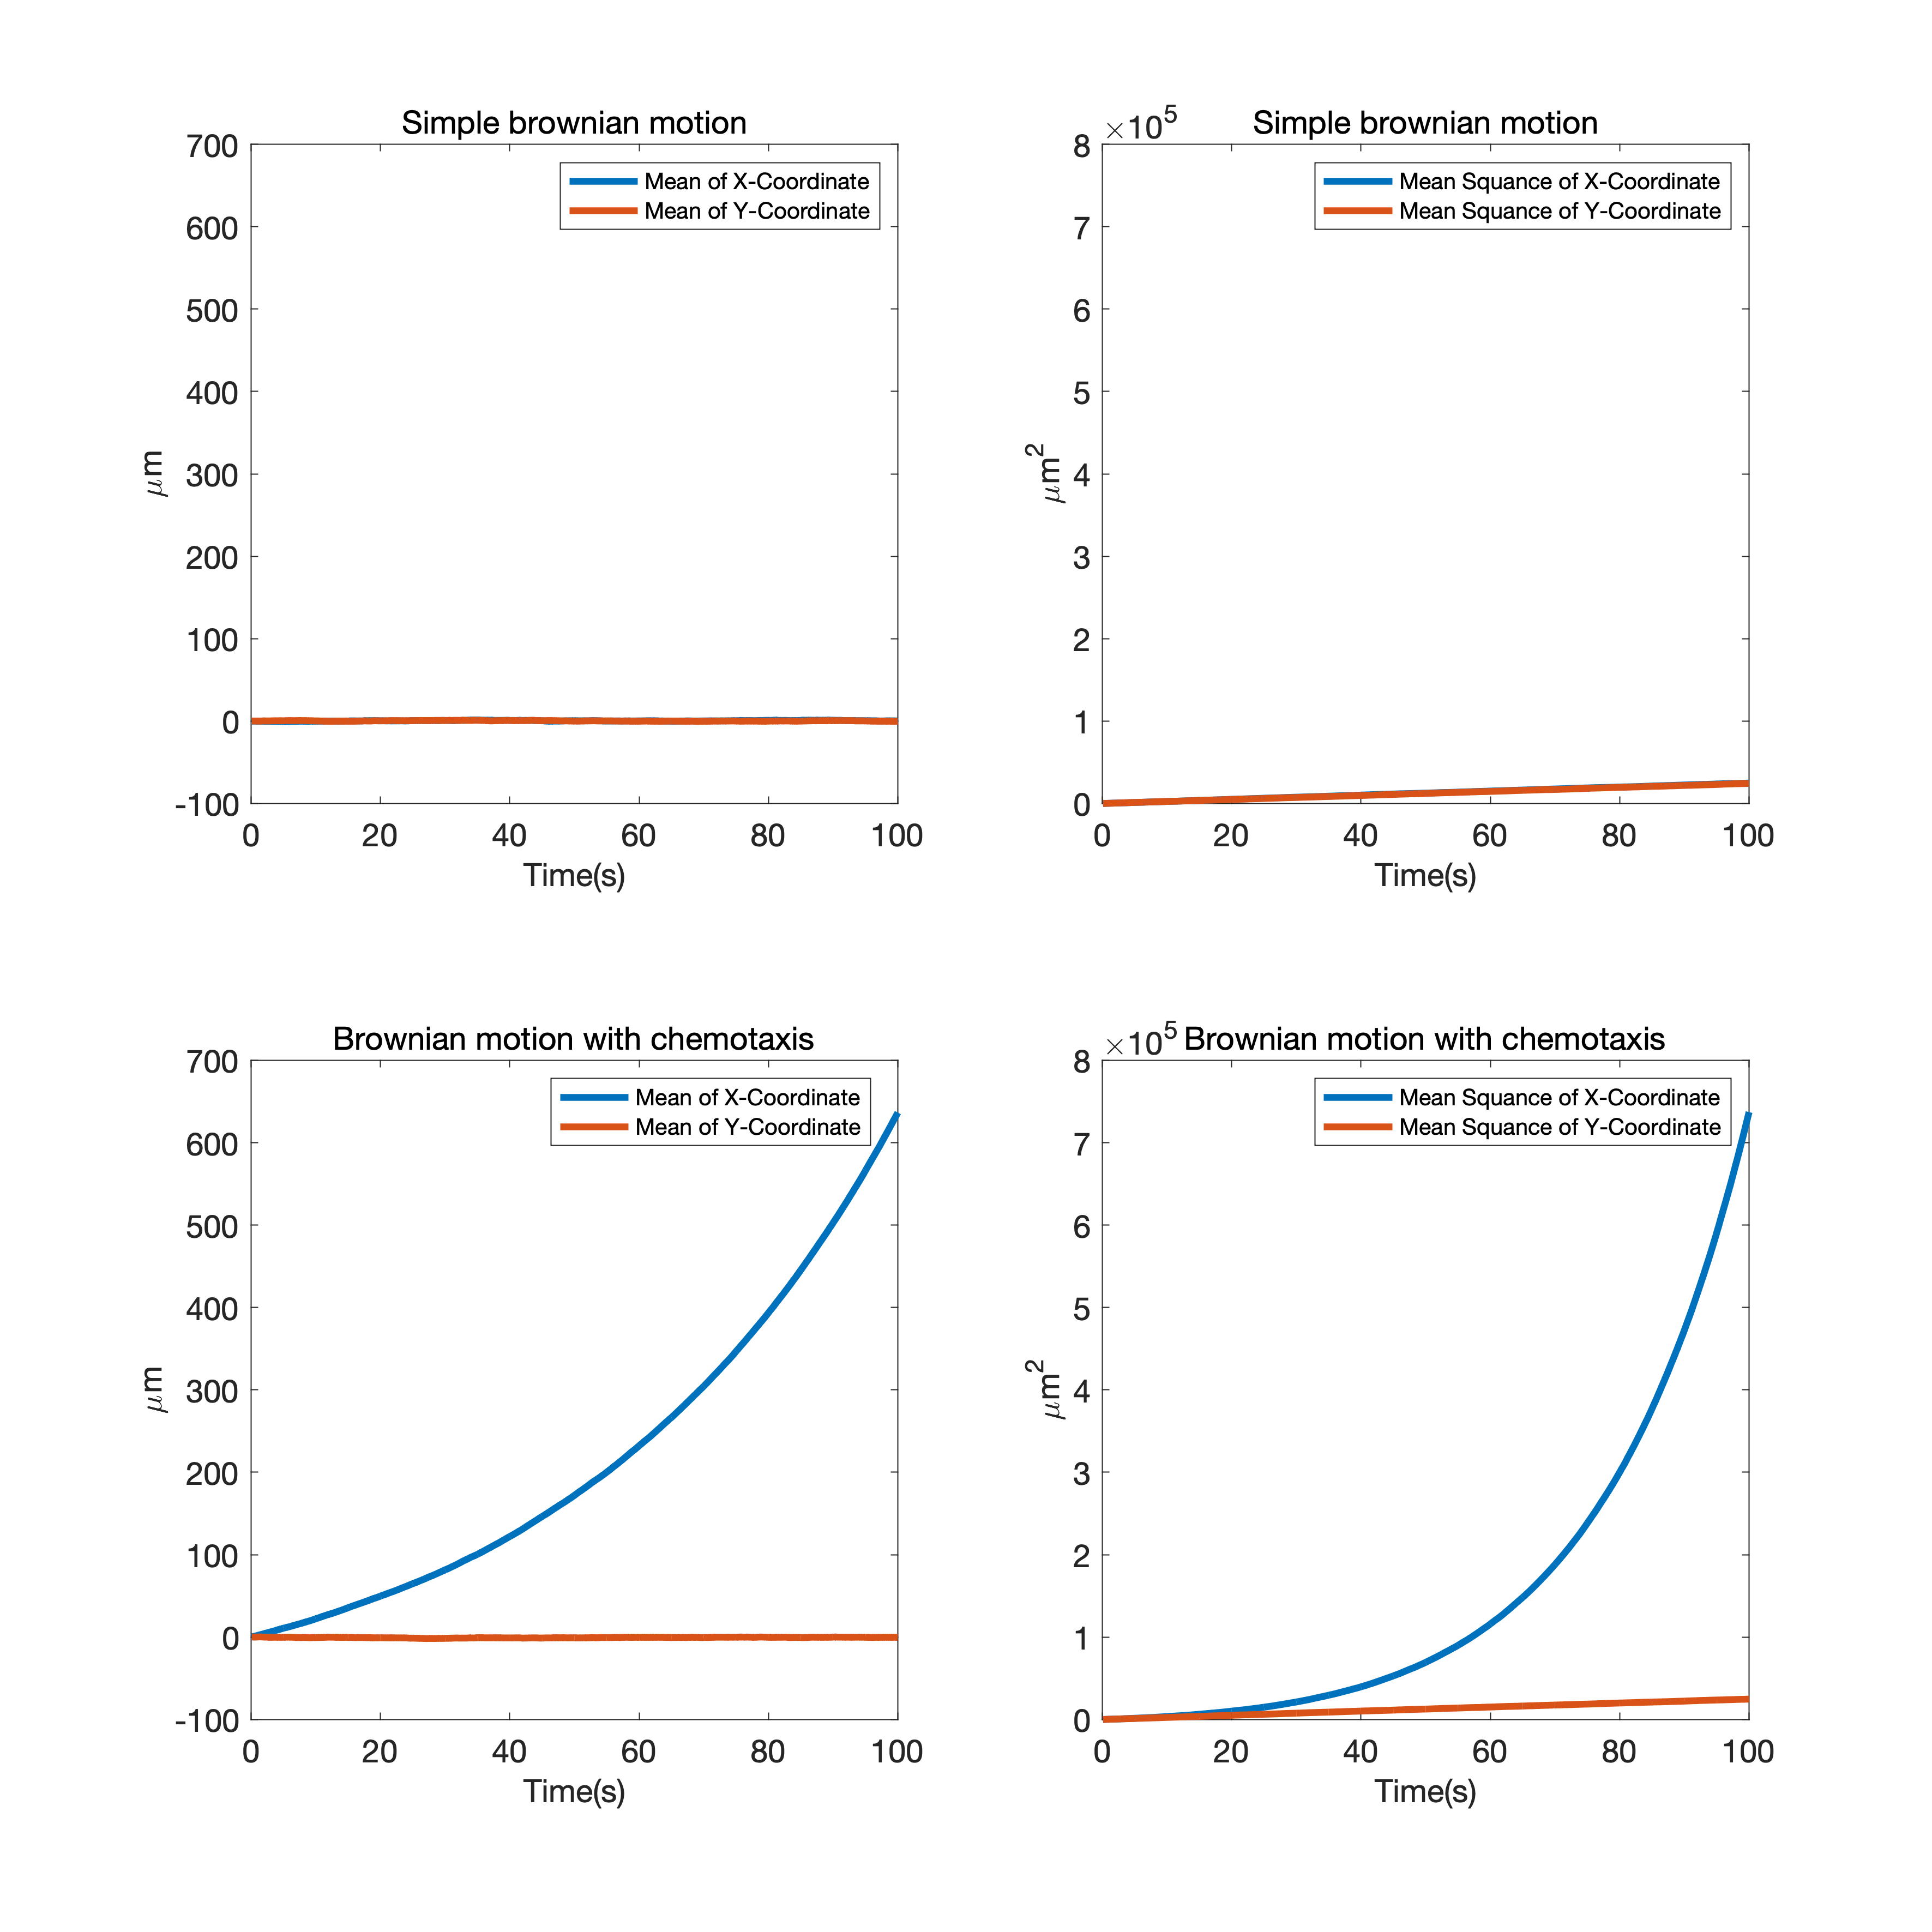
\includegraphics[width=1\linewidth]{Figures/P2_fig4.png}
\caption{compare the ``mean displacement'' and ``mean displacement-square'' overtime between ``simple Brownian motion'' with ``Brownian motion with chemotaxis in x-direction'' for 10000 cells.}
\label{P2_fig4}
\end{figure}

\newpage
The simple 2D Brownian motion shows the random movement of the cells, both ”mean displacement” and ”mean displacement-square” show no distinct changes.
While the simple model simulation shows the chemoattractant’s influence on the E.coli motion, the ”mean displacement” and ”mean displacement-square” on X-direction are extremely increased. It really shows the chemotaxis’s influence on the movement of E.coli, but it has no much biological meanings.


%----------------------------------------------------------------------------------------



%----------------------------------------------------------------------------------------




%The \code{biblatex} package is used to format the bibliography and inserts references such as this one \parencite{Reference1}. The options used in the \file{main.tex} file mean that the in-text citations of references are formatted with the author(s) listed with the date of the publication. Multiple references are separated by semicolons (e.g. \parencite{Reference2, Reference1}) and references with more than three authors only show the first author with \emph{et al.} indicating there are more authors (e.g. \parencite{Reference3}). This is done automatically for you. To see how you use references, have a look at the \file{Chapter1.tex} source file. Many reference managers allow you to simply drag the reference into the document as you type.

